\section{Method}
\label{sec:method}

Our pipeline decomposes video object removal into two stages: \emph{dynamic mask
extraction} and \emph{background inpainting}. We evaluate a sequence of routes that
isolate mask generation, mask refinement, geometry priors, and generative inpainting.
An overview is shown in Figure~\ref{fig:pipeline}.

\begin{figure*}[t]
  \centering
  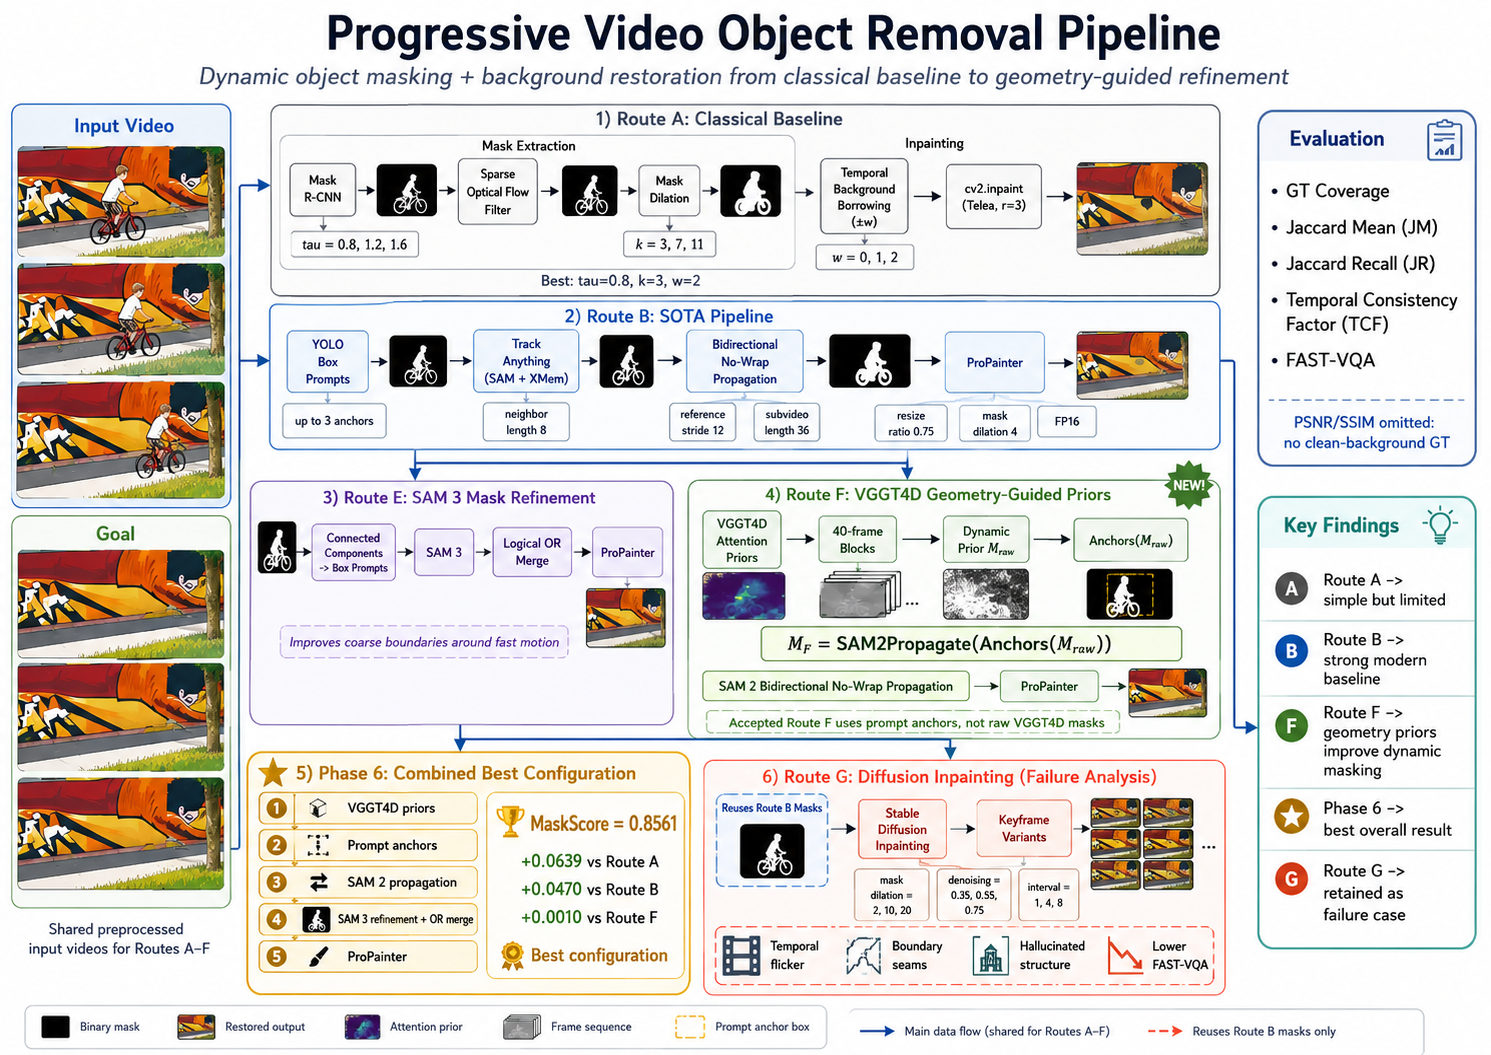
\includegraphics[width=\textwidth]{figures/fig_pipeline.png}
  \caption{Overview of our video object removal pipeline. Routes A--F share the same
  preprocessed input videos. Route~G reuses Route~B masks and changes only the
  inpainting module, so it is analyzed as a failure case rather than ranked as a main
  method.}
  \label{fig:pipeline}
\end{figure*}

\subsection{Route A: Classical Baseline}
\label{sec:method:a}

\paragraph{Mask Extraction.}
We apply Mask R-CNN~\cite{maskrcnn} (ResNet-50-FPN-v2 backbone) to extract per-frame
instance masks for dynamic classes such as \emph{person}, \emph{bicycle}, and
\emph{car}.
To filter static detections, we compute sparse Lucas-Kanade optical flow on
Shi-Tomasi corner features inside each mask and discard instances whose mean flow
magnitude falls below threshold $\tau \in \{0.8, 1.2, 1.6\}$~px/frame.
Mask dilation $k \in \{3,7,11\}$ is then ablated to cover motion blur while controlling
background leakage.

\paragraph{Inpainting.}
We first attempt \emph{temporal background borrowing}: for each masked pixel, we search
a temporal window of $\pm w \in \{0,1,2\}$ frames for a clean pixel at the same
location. Remaining holes are filled with \texttt{cv2.inpaint} (Telea algorithm,
radius~3~px). The best configuration uses $\tau{=}0.8$, dilation $k{=}3$, and
$w{=}2$.

\subsection{Route B: SOTA Pipeline}
\label{sec:method:b}

\paragraph{Mask Extraction.}
Track Anything~\cite{trackanything} (SAM + XMem memory) is initialized with
YOLO-derived bounding-box prompts on up to 3 anchor frames, selected by connected-component
analysis with a minimum inter-anchor interval of $16\%$ of total frames.
We adopt \emph{bidirectional no-wrap} propagation: forward pass from each anchor,
then backward pass, without wrapping at video boundaries.

\paragraph{Inpainting.}
ProPainter~\cite{propainter} takes frames and binary masks as input.
Its dual-domain propagation first completes optical flow fields, then propagates
features across frames. The selected Route~B configuration uses neighbor length~8,
reference stride~12, subvideo length~36, resize ratio~0.75, mask dilation~4, and
FP16 inference.

\subsection{Route E: SAM~3 Mask Refinement}
\label{sec:method:e}

Route~B masks exhibit coarse boundaries around fast-moving objects.
We introduce a SAM~3~\cite{sam3} refinement step. For each input mask sequence, connected
components are converted into relative-coordinate box prompts on up to 3 anchor frames;
SAM~3 then propagates each anchor forward and backward without wrap-around. The refined
mask is merged with the input mask by logical OR before ProPainter inpainting. Wild is
excluded from the SAM~3 refinement stage because it has no GT mask for mask-score
selection, but final videos are still generated for it.

\subsection{Route F: VGGT4D Geometry-Guided Priors}
\label{sec:method:f}

VGGT4D~\cite{vggt4d} mines motion cues from VGGT~\cite{vggt} attention maps via
Gram similarity matrices, producing per-frame dynamic probability maps without
any fine-tuning. We process the video in blocks of 40 frames and obtain a
\emph{dynamic prior mask} $M_{\text{raw}}$. The accepted Route~F run does not use this
raw mask directly and does not fuse it with Track Anything as the final result. Instead,
connected components in $M_{\text{raw}}$ are converted to prompt anchors using the same
anchor policy as Route~B. These prompts are then propagated by the mask backend not
selected by Route~B. Since Route~B selected Track Anything, Route~F's final backend is
SAM~2:
\begin{equation}
  M_{\text{F}} = \mathrm{SAM2Propagate}(
  \mathrm{Anchors}(M_{\text{raw}})).
  \label{eq:vggt_prompt}
\end{equation}
We also evaluated the raw VGGT4D replacement and bidirectional flow/trajectory fusion
variants, but global non-oracle MaskScore selected the SAM~2 alternate-backend result.
This distinction is important: raw VGGT4D masks over-cover the target region and obtain
low IoU, whereas prompt-conditioned SAM~2 propagation converts the geometry prior into a
usable dynamic-object mask.

\subsection{Phase~6: Combined Best Configuration}
\label{sec:method:phase6}

Our best configuration applies Route~E's SAM~3 refinement to the accepted Route~F mask:
\begin{enumerate}
  \item VGGT4D dynamic prior generation (40-frame blocks).
  \item Conversion of VGGT4D prior masks to prompt anchors.
  \item SAM~2 bidirectional no-wrap propagation, because SAM~2 is the alternate backend to Route~B's Track Anything.
  \item SAM~3 boundary refinement with logical-OR merge against the Route~F mask.
  \item ProPainter inpainting.
\end{enumerate}
This achieves MaskScore~$=0.8561$, an absolute $+0.0639$ gain over Route~A and a small
$+0.0010$ gain over Route~F.

\subsection{Route G: Diffusion Inpainting (Failure Analysis)}
\label{sec:method:g}

We explore Stable Diffusion~\cite{ldm} inpainting as an alternative local renderer under
fixed Route~B masks. Four variants sweep mask dilation $\in\{2,10,20\}$~px, denoising
strength $\in\{0.35,0.55,0.75\}$, and keyframe interval $\in\{1,4,8\}$.
All variants preserve Route~B's mask metrics by construction. They reduce TCF in some
settings because keyframe propagation reuses fewer independently sampled diffusion
frames, but visual inspection shows temporal flicker, boundary seams, and hallucinated
background structure.
We conclude that frame-level diffusion inpainting is unsuitable for video without
explicit temporal conditioning; results are retained as failure cases
(Section~\ref{sec:exp}).
